\section{Data Flow Diagram}
\label{sec:data-flow-diagram}

\subsection{Level 0}

\begin{figure}[h!]
	\begin{centering}
		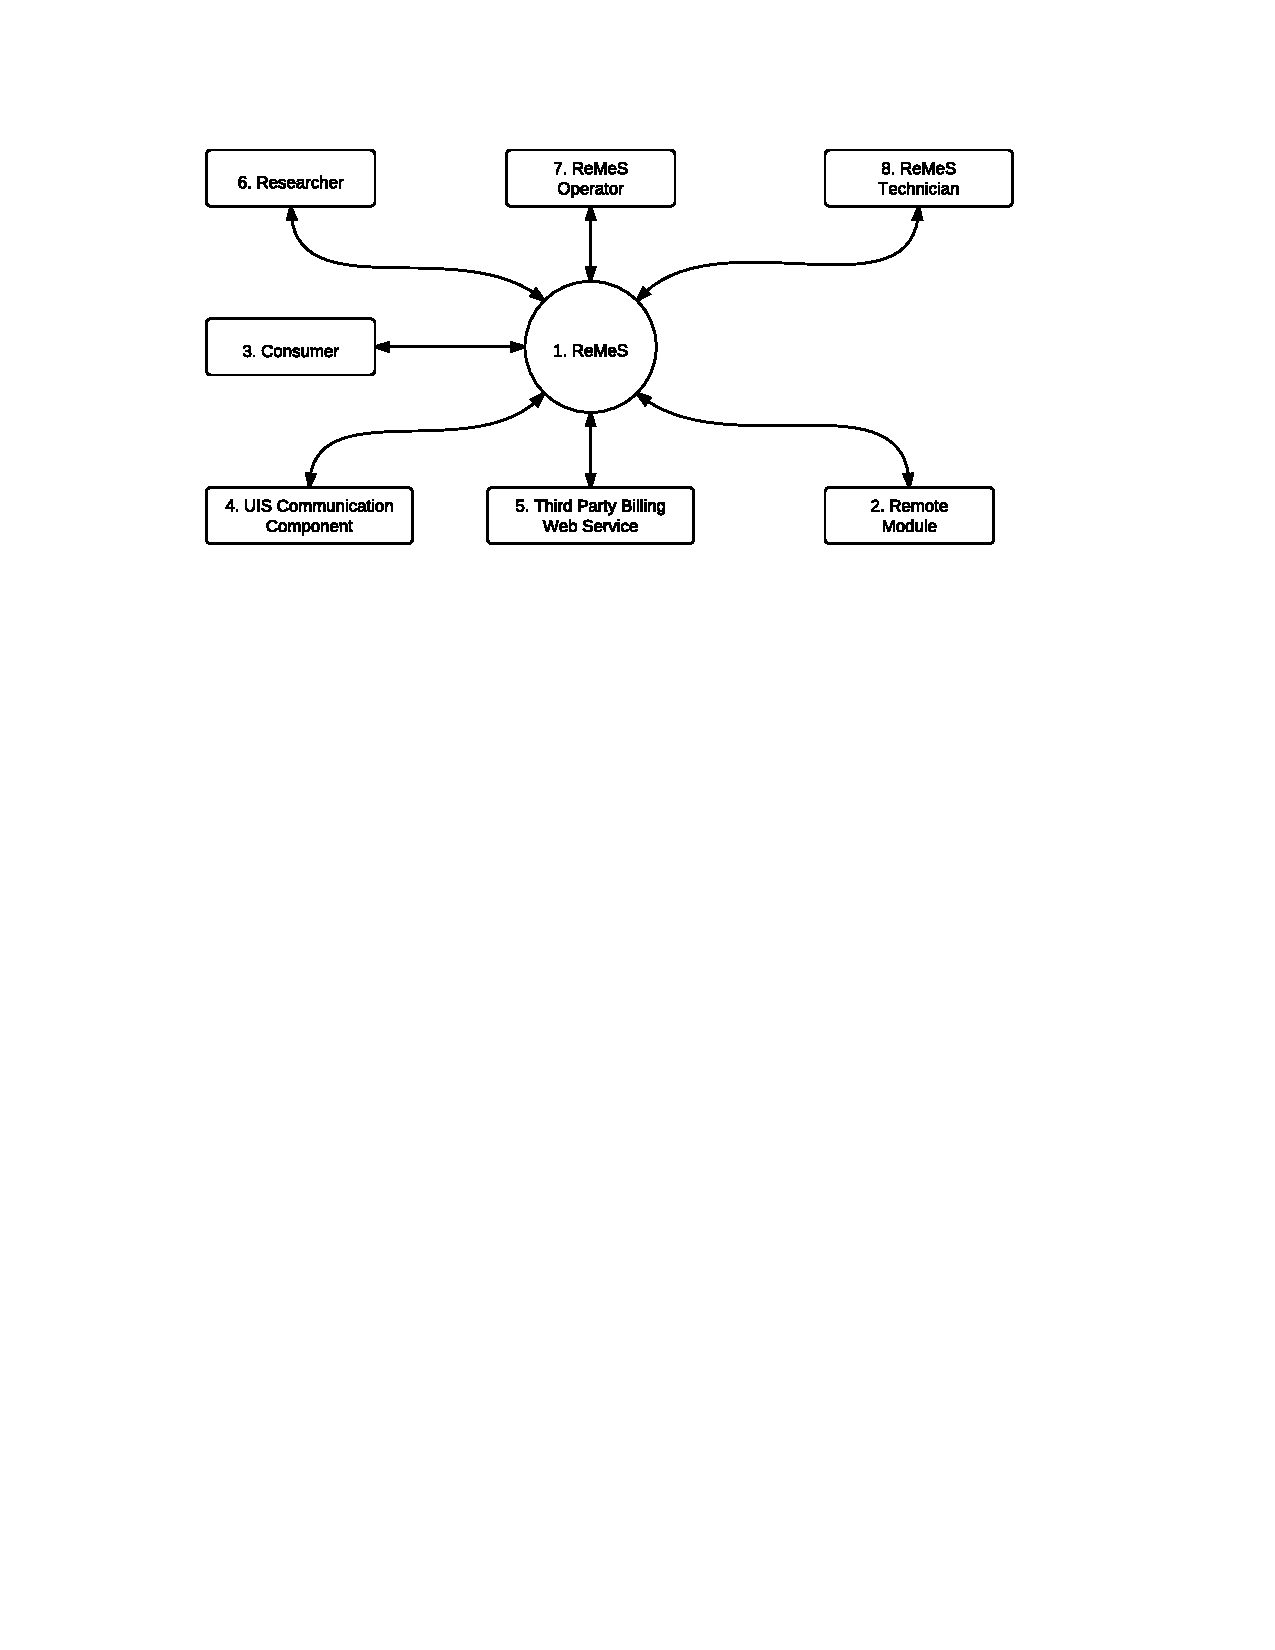
\includegraphics[width=0.8\textwidth]{figs/level-0.pdf}
		\caption{The level zero data flow diagram of the ReMeS system.}
		\label{fig:data-flow-diagram-lvl0}
	\end{centering}
\end{figure}

\npar In figure \ref{fig:data-flow-diagram-lvl0} the level zero data flow
diagram (DFD) is depicted. It is a representation of the whole system and is
quite analogous to the context diagram. There is only one process, ReMeS, and
all actors are derived from the context diagram. 

\subsection{Level 1}

\begin{figure}[h!]
	\begin{centering}
		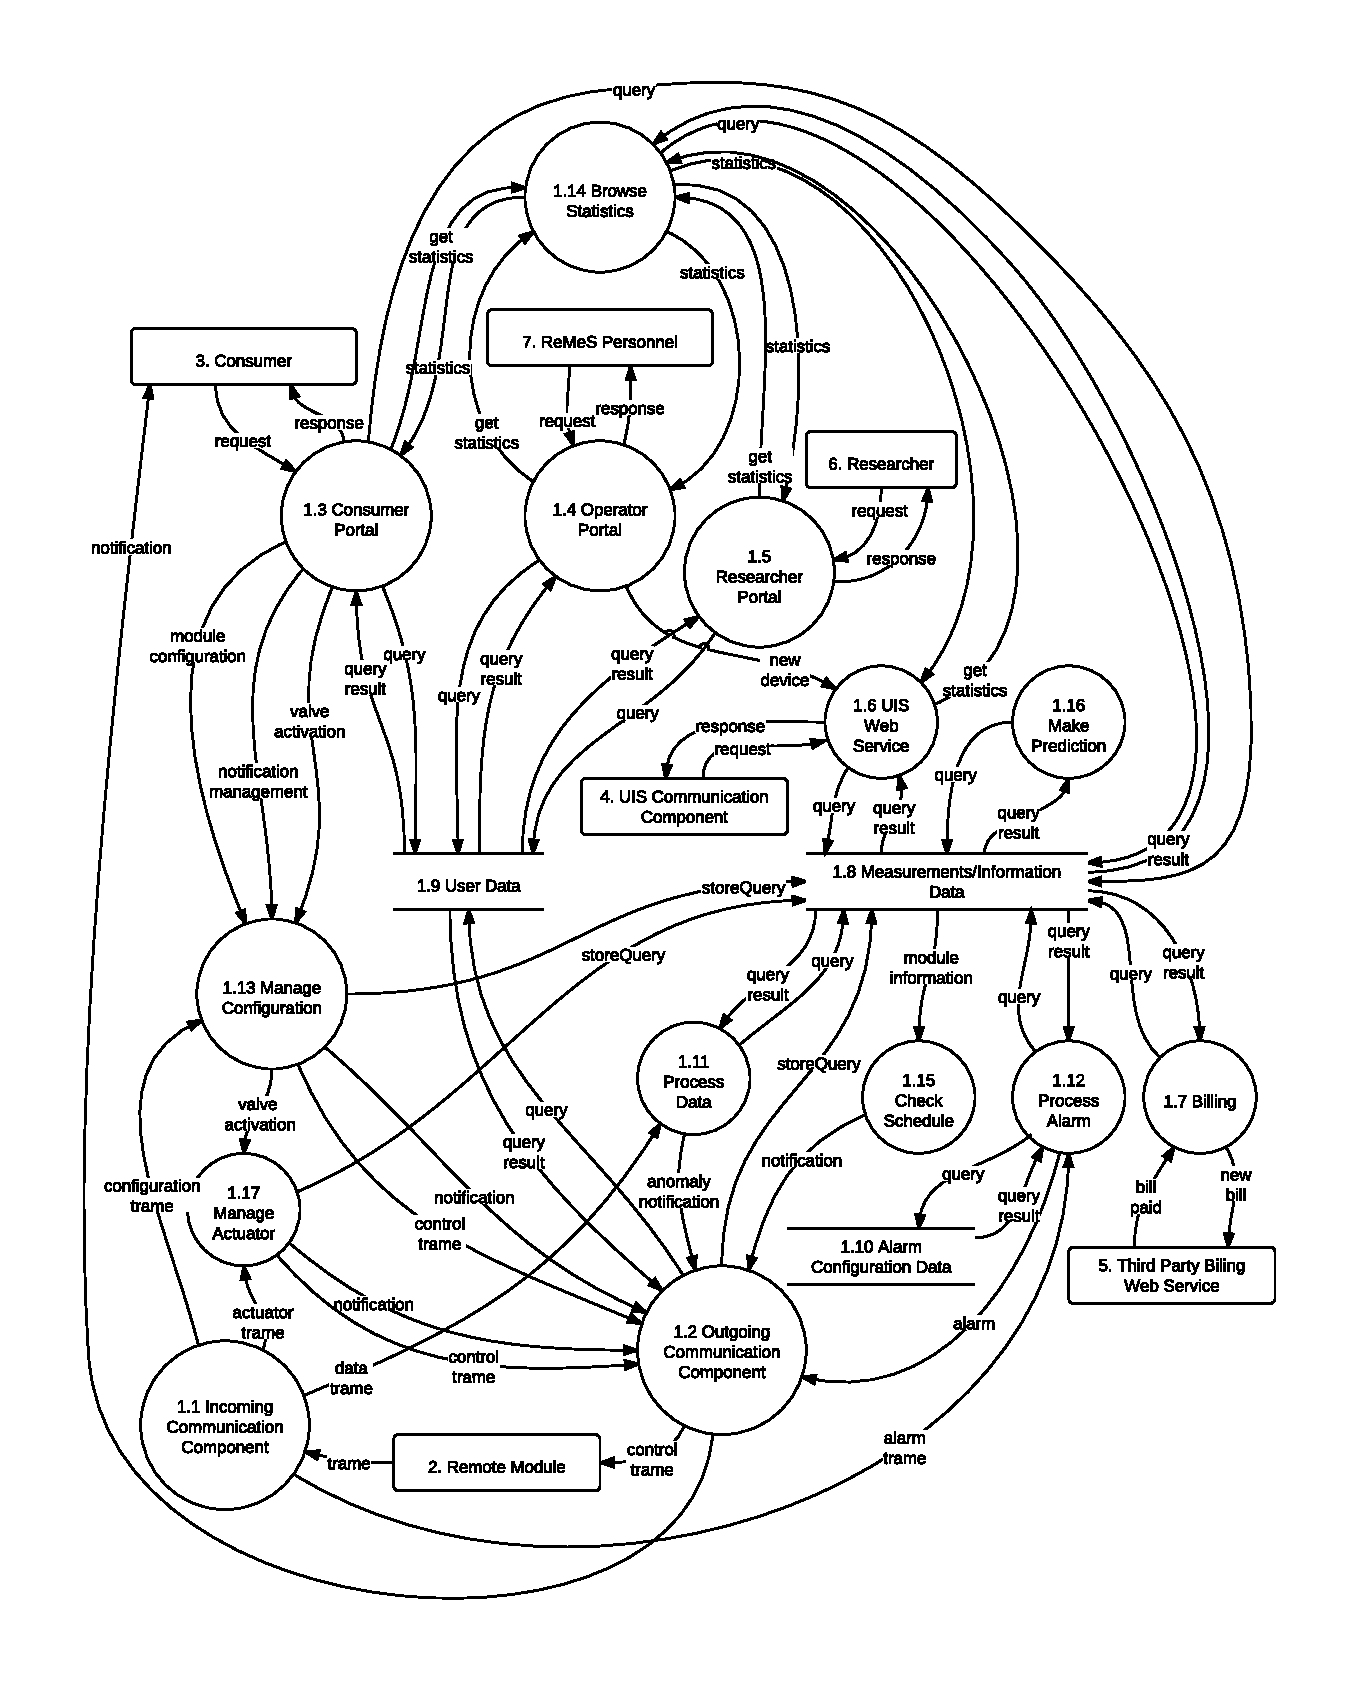
\includegraphics[width=\textwidth]{figs/level-1.pdf}
		\caption{The most detailed data flow diagram of the ReMeS system, namely level
		one.}
		\label{fig:data-flow-diagram-lvl2}
	\end{centering}
\end{figure}

\npar In the next level, the single ReMeS process is decomposed. The
decomposition follows from the component diagram. The result is shown in figure
\ref{fig:data-flow-diagram-lvl2}.

\npar Notice that the ``Data Processor'' and ``Anomaly Detector'' are not
present in the diagram. Because the Data Processor hands over all trames 
to the Anomaly Detector and the latter's service is only used by the Data
Processor, they are merged into a single ``Process Data'' process.

\npar It is also important to remark that ReMeS operator and ReMeS technician
are generalised into ReMeS personnel. This is done because there is no
significant difference between the two from the system's point of view. They
both only communicate with the Operator Portal.

\npar The database component from the component diagram is also decomposed into
different data stores: Measurements and Information Data, User Data and Alarm
Configuration Data.


